% Drawing 8/03-3 -- folder 8, batch 03, archive page 59 (PDF page 60).
% Transcription: même papier, tenu en hauteur, au crayon. En haut : un axe horizontal de seize carreaux, deux droites issues de l'origine et du point $(1, 0)$ qui se rejoignent à l'abscisse 16, des points marqués le long. En bas : d'une seconde origine et du point voisin partent cinq droites de pentes décroissantes, la plus haute épaisse et brisée au départ, aboutissant à une verticale d'abscisse 16 marquée de points.
% Kind: two pencil graphs on squared paper (pencils of lines of rational slopes). Method 2 (schematic redraw from the facsimile). Status: partial.
% Notes: Pencil on the same paper held upright. Upper graph, on a computed lattice (one square = 4.6 units): the horizontal axis of 16 squares, a short vertical tick at the origin, a thin line from the origin and a heavy line from (1, 0) meeting at abscissa 16 (height about 13), the short segment from the origin to (2, 1), seven marked points. Lower graph: the vertical at abscissa 16 with its dots; from the origin a heavy line, broken at its start, to height about 11, and four more lines to heights about 8, 7, 4 and 2; each is doubled by a faint line from the neighbouring point (1, 0); one faint line overshoots the vertical. Left out: the fractions written on the page (text), the ruling, several further faint lines of the lower pencil between the first and the third line, and faint lattice dots. Still differs: the note of the transcription counts six lines in the lower pencil, five directions are drawn here (the faint ones between are not separated on a 200 dpi render); the end heights are approximate. Overlaid 2026-11-12 (Opus 5.5) on a 300 dpi colour render: the upper graph, the end heights of the lower pencil and the dots of the vertical match the page within about half a unit; in the lower pencil the heavy line from the origin is straighter on the page than drawn (the broken course via the third square is a fainter stroke) and the line from (1, 0) to the heavy end runs about 1 unit low near its start. Not corrected further. Redrawn 2026-11-12 (issue 128): to check again.
% Coordinates: 1 unit = 1 mm = 1/100 of the crop width (bbox in page fractions: [0.09, 0.068, 0.97, 0.875]).
% Redrawn by Claude (claude-fable-5-2), issue #128, 2026-11-12; not checked by a human; not compiled (no TeX in the session).
% Overlaid by Claude (claude-opus-5-5) 2026-11-12 (issue #128): rasterised from its own coordinates over the colour facsimile and checked or corrected. Not compiled. Status: partial.
% Rights: reproduces part of the work -- behind RENDER_TRANSCRIPTS, never published by itself.
\documentclass[tikz,border=3pt]{standalone}
\usepackage{amsmath,amssymb}
\usetikzlibrary{patterns,arrows.meta}
\tikzset{pencil/.style={black!45}, struck/.style={black!35}, mpt/.style={circle,draw,inner sep=1.3pt}, pt/.style={circle,fill,inner sep=0.9pt}, opt/.style={circle,draw,fill=white,inner sep=1.1pt}}
\begin{document}
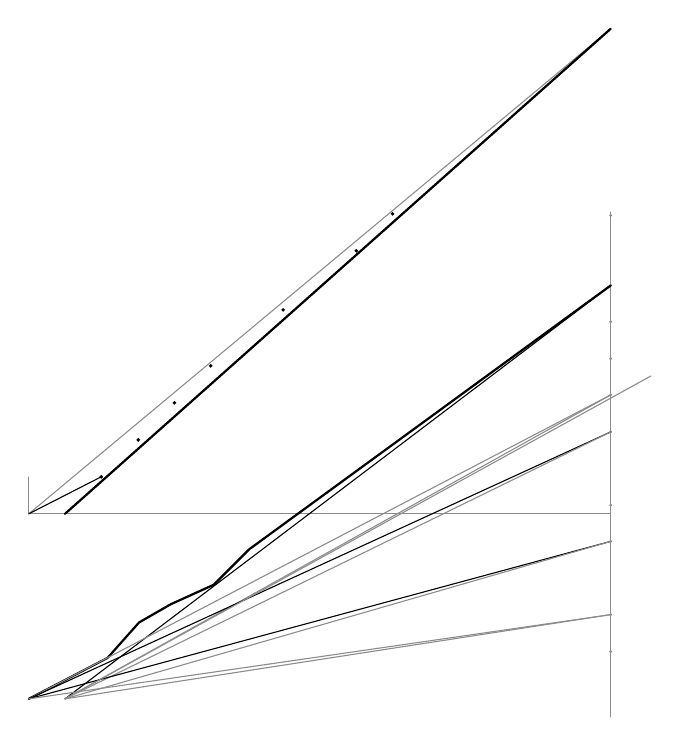
\begin{tikzpicture}[x=1mm,y=1mm,line cap=round,line join=round,font=\small]
\draw[pencil] (4,-84) -- (77.9,-84);
\draw[pencil] (4,-84) -- (4,-79.3);
\draw[pencil] (4,-84) -- (77.9,-22.4);
\draw[thick] (8.6,-84) -- (77.9,-22.4);
\draw (4,-84) -- (13.2,-79.3);
\node[pt,inner sep=0.5pt] at (13.2,-79.3) {};
\node[pt,inner sep=0.5pt] at (17.9,-74.6) {};
\node[pt,inner sep=0.5pt] at (22.5,-69.9) {};
\node[pt,inner sep=0.5pt] at (27.1,-65.2) {};
\node[pt,inner sep=0.5pt] at (36.3,-58.1) {};
\node[pt,inner sep=0.5pt] at (45.6,-50.6) {};
\node[pt,inner sep=0.5pt] at (50.2,-45.9) {};
\draw[pencil] (77.9,-109.8) -- (77.9,-45.7);
\node[pt,pencil,inner sep=0.4pt] at (77.9,-101.5) {};
\node[pt,pencil,inner sep=0.4pt] at (77.9,-96.8) {};
\node[pt,pencil,inner sep=0.4pt] at (77.9,-87.5) {};
\node[pt,pencil,inner sep=0.4pt] at (77.9,-82.9) {};
\node[pt,pencil,inner sep=0.4pt] at (77.9,-73.6) {};
\node[pt,pencil,inner sep=0.4pt] at (77.9,-68.9) {};
\node[pt,pencil,inner sep=0.4pt] at (77.9,-64.3) {};
\node[pt,pencil,inner sep=0.4pt] at (77.9,-59.6) {};
\node[pt,pencil,inner sep=0.4pt] at (77.9,-55) {};
\node[pt,pencil,inner sep=0.4pt] at (77.9,-46.1) {};
\draw[thick] (4,-107.5) -- (14,-102.3) -- (18,-97.8) -- (22,-95.5) -- (27.5,-93) -- (32,-88.5) -- (77.9,-55);
\draw (8.6,-107.5) -- (77.9,-55);
\draw[pencil] (4,-107.5) -- (77.9,-68.9);
\draw[pencil] (8.6,-107.5) -- (77.9,-68.9);
\draw (4,-107.5) -- (77.9,-73.6);
\draw[pencil] (8.6,-107.5) -- (77.9,-73.6);
\draw (4,-107.5) -- (77.9,-87.5);
\draw[pencil] (8.6,-107.5) -- (77.9,-87.5);
\draw[pencil] (4,-107.5) -- (77.9,-96.8);
\draw[pencil] (8.6,-107.5) -- (77.9,-96.8);
\draw[pencil] (8.6,-107.5) -- (83,-66.5);
\end{tikzpicture}
\end{document}
